%
% File: chap01.tex
% Author: Liam O'Shea
% Description: Introduction chapter where the boxing goes.
%
\let\textcircled=\pgftextcircled
\chapter{Implementation}
\label{chap:intro}

\initial{E}ach individual implementation stage will be discussed, collection of data, dimensionality reduction, punch segmentation, punch classification and quality assessment.  



%=======
My first step was to organise the data in such a way that it could be usefully visualised so that I comprehend the nature of the data that needed to be processed. I began by recording a sequence of 5 jabs, being careful to evenly time the punches before manually isolating the left wrist joint over time. As my jab was thrown 5 times with approximately equal spacing I was hoping that I would be able to produce a sinusoidal-like sequence with five full `cycles' demonstrating the movement of the left hand over time.\newline

\begin{figure}[h]
    \centering
    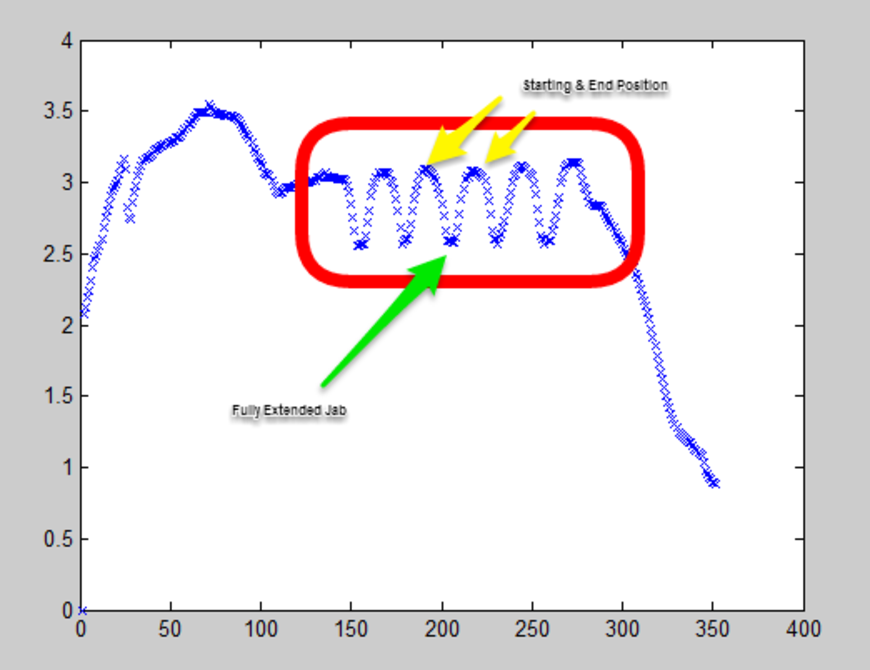
\includegraphics[height=0.25\textheight]{fig04/lwrist.pdf}
    \mycaption[Left wrist joint over time]{This figure shows the left wrist joints movement in the Z direction over time. The x-axis represents the kinect frames, they y-axis the distance of the fist from the kinect. }
    \label{fig:kinect}
\end{figure}

SO MANY REASONS WHY JUST ONE HAND IS SHIT
POSE, whole body, not robust etc...

I needed to find a sensible way to visualise the entire skeleton over time in a meaningful way. I naively began by plotting the entire data set which produced a fairly jagged signal with two troughs followed by a massive peak before levelling of again. At this point I realised attempting to plot the skeleton data in this way would not be meaningful but as a test I differentiated the raw data to produce velocity as opposed to distance, I was hoping that this might show something more meaningful or smooth out the data.
Realising that for now I needed to look at individual joints I took the central hip joint and plotted it's movement in the Z direction over time as well as plotting the differential of that to give me the velocity. As you can see from Figure 3.1, the velocity data was much more useful and produced a reasonably smooth periodic sequence. Since the initial recording was 10 jabs one after the other I expected a periodic, cyclical signal to be produced.

\begin{figure}[h]
\centering
\begin{minipage}{6.0cm}
    \centering
    \subtop[]{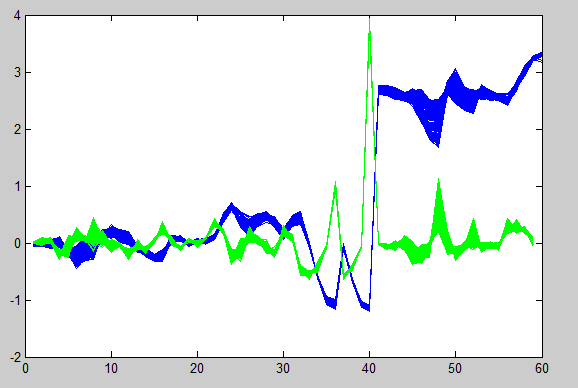
\includegraphics[height=0.25\textheight]{fig04/fig06}}
    \label{fig:1}
\end{minipage}
\begin{minipage}{6.0cm}
    \centering
    \subtop[]{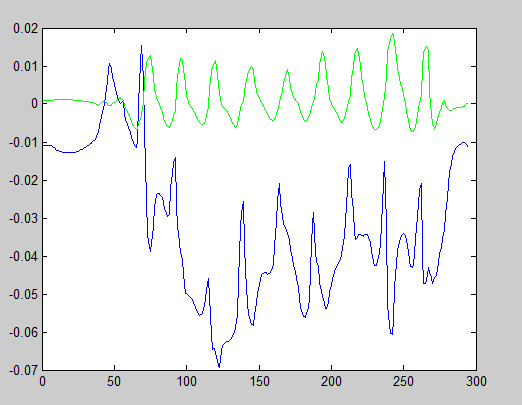
\includegraphics[height=0.25\textheight]{fig04/fig07}}
    \label{fig:2}
\end{minipage}
\mycaption[ALLData] {(a) Kinect Skeleton vs Time. 
(b) Hip Joint vs Time, Blue = Raw data, Green = Differentiated data.}
\end{figure}

Since PCA was a familiar method I implemented it in Matlab with 3 principal components and plotted the first project coefficient for the first principal component with both the distance and velocity data. From this we can see that the distance data was slightly jagged with a local maxima which might obstruct attempts to automatically segment punches. The velocity data produced a smoother series but introduced unwanted noise towards the beginning and end of a sequence.

\begin{figure}[h]
\centering
\begin{minipage}{6.0cm}
    \centering
    \subtop[]{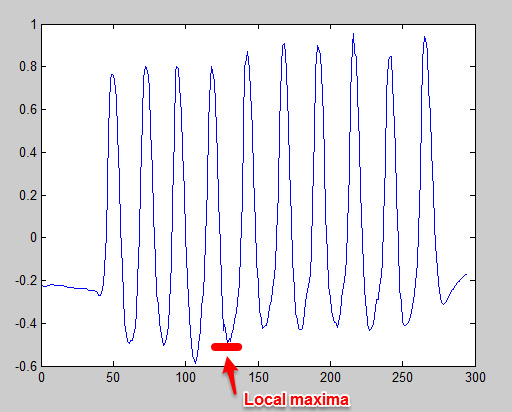
\includegraphics[height=0.25\textheight]{fig04/fig02}}
    \label{fig:1}
\end{minipage}
\begin{minipage}{6.0cm}
    \centering
    \subtop[]{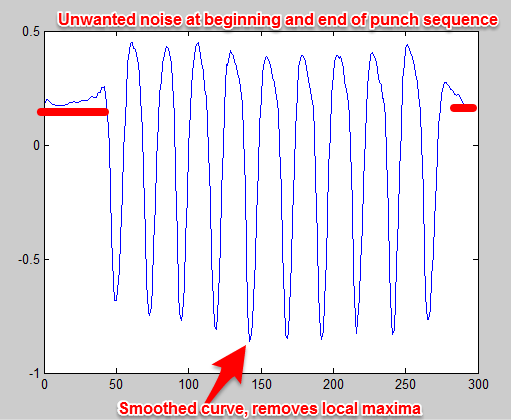
\includegraphics[height=0.25\textheight]{fig04/fig03}}
    \label{fig:2}
\end{minipage}
\mycaption[ALLData] {(a) Kinect Skeleton vs Time. 
(b) Hip Joint vs Time, Blue = Raw data, Green = Differentiated data.}
\end{figure}




\begin{wrapfigure}{R}{0.50\textwidth}
% \vspace{-15pt}
% \hspace{15pt}
\begin{center}
    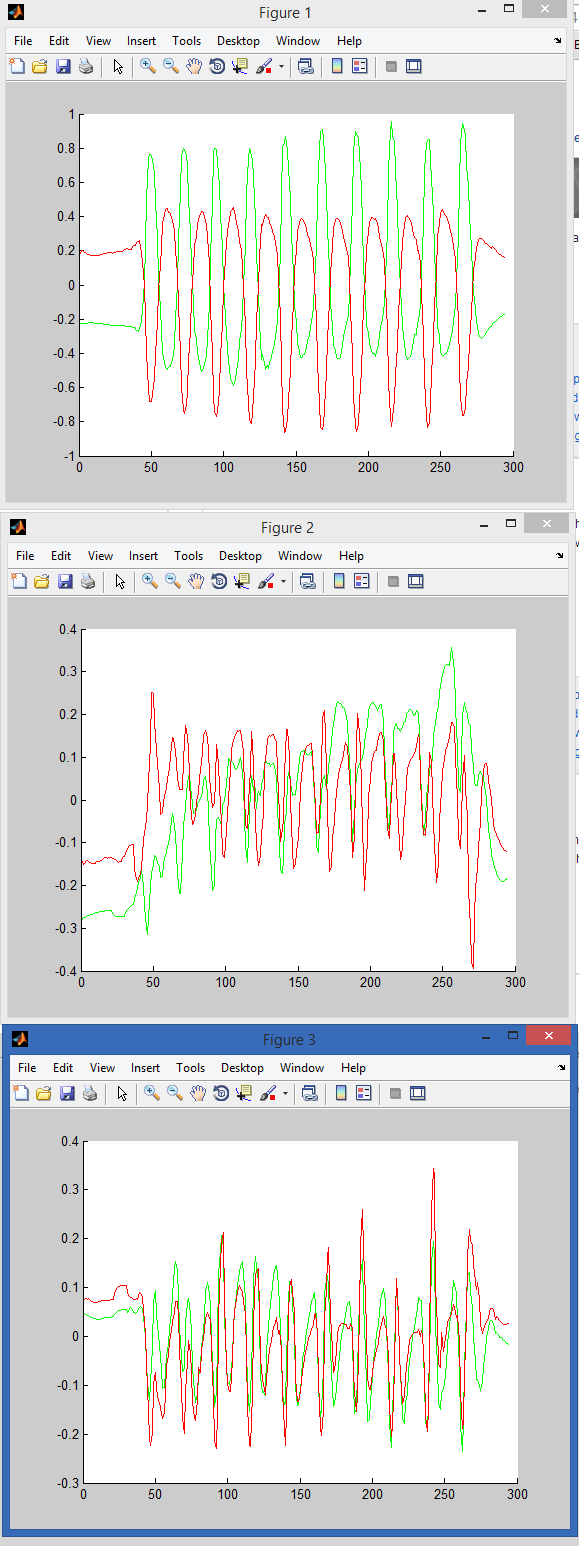
\includegraphics[width=0.48\textwidth]{fig04/3pcs.png}
    \caption{SOME CAPTION}
    \label{fig:WHAT}
\end{center}
% \vspace{}
% \vspace{}
\end{wrapfigure}
Next I plotted all three projection coefficients for the three principal components for both distance and velocity. We can see for the first projection coefficient both distance and velocity are similar with distance being slightly more jagged at the peaks of the punching period and velocity being more jagged at the start and end.
For the second they are both fairly similar but with distance having less peaks and troughs and with only one dramatic spike at 250 as opposed to two at 50 and 275.
For the third the depth comes out ahead with a smoother signal which again has less `spikes' (which will make it hard to segment.) Although by eye it looks like the depth data under PCA produces a more useful periodic type wave neither are convincing and we should do some comparisons.


\paragraph {Dimensionality Reduction Comparison}
Each dimensionality reduction method was evaluated on it's ability to produce useful, smooth and sinusoidal output to aid automatic segmentation. Automatic segmentation is a crucial step in the project since on a larger scale much greater data sets will need to be used and collated from multiple sources. If these can be processed and automatically segmented this will remove any manual work required and make this a truly useful system. I used the Matlab Dimensionality Toolbox and the `intrinsic_dim' function that performs an estimation of the intrinsic dimensionality of a dataset X given a specific method. This was calculated six different methods, maximum-likelihood estimation (MLE), correlation dimension estimation (CorrDim), nearest neighbourhood, packing numbers and Geodesic minimum spanning tree (GMST) and eigenvalue estimation.
These results were then combined and averaged to produce a dimension {\bf d} to be used as an argument for LLE, LLE with d, Laplacian, LTSA, CCA and PCA (see background). The lower dimensionality data was then plotted and analysed.

\begin{figure}[h]
    \centering
    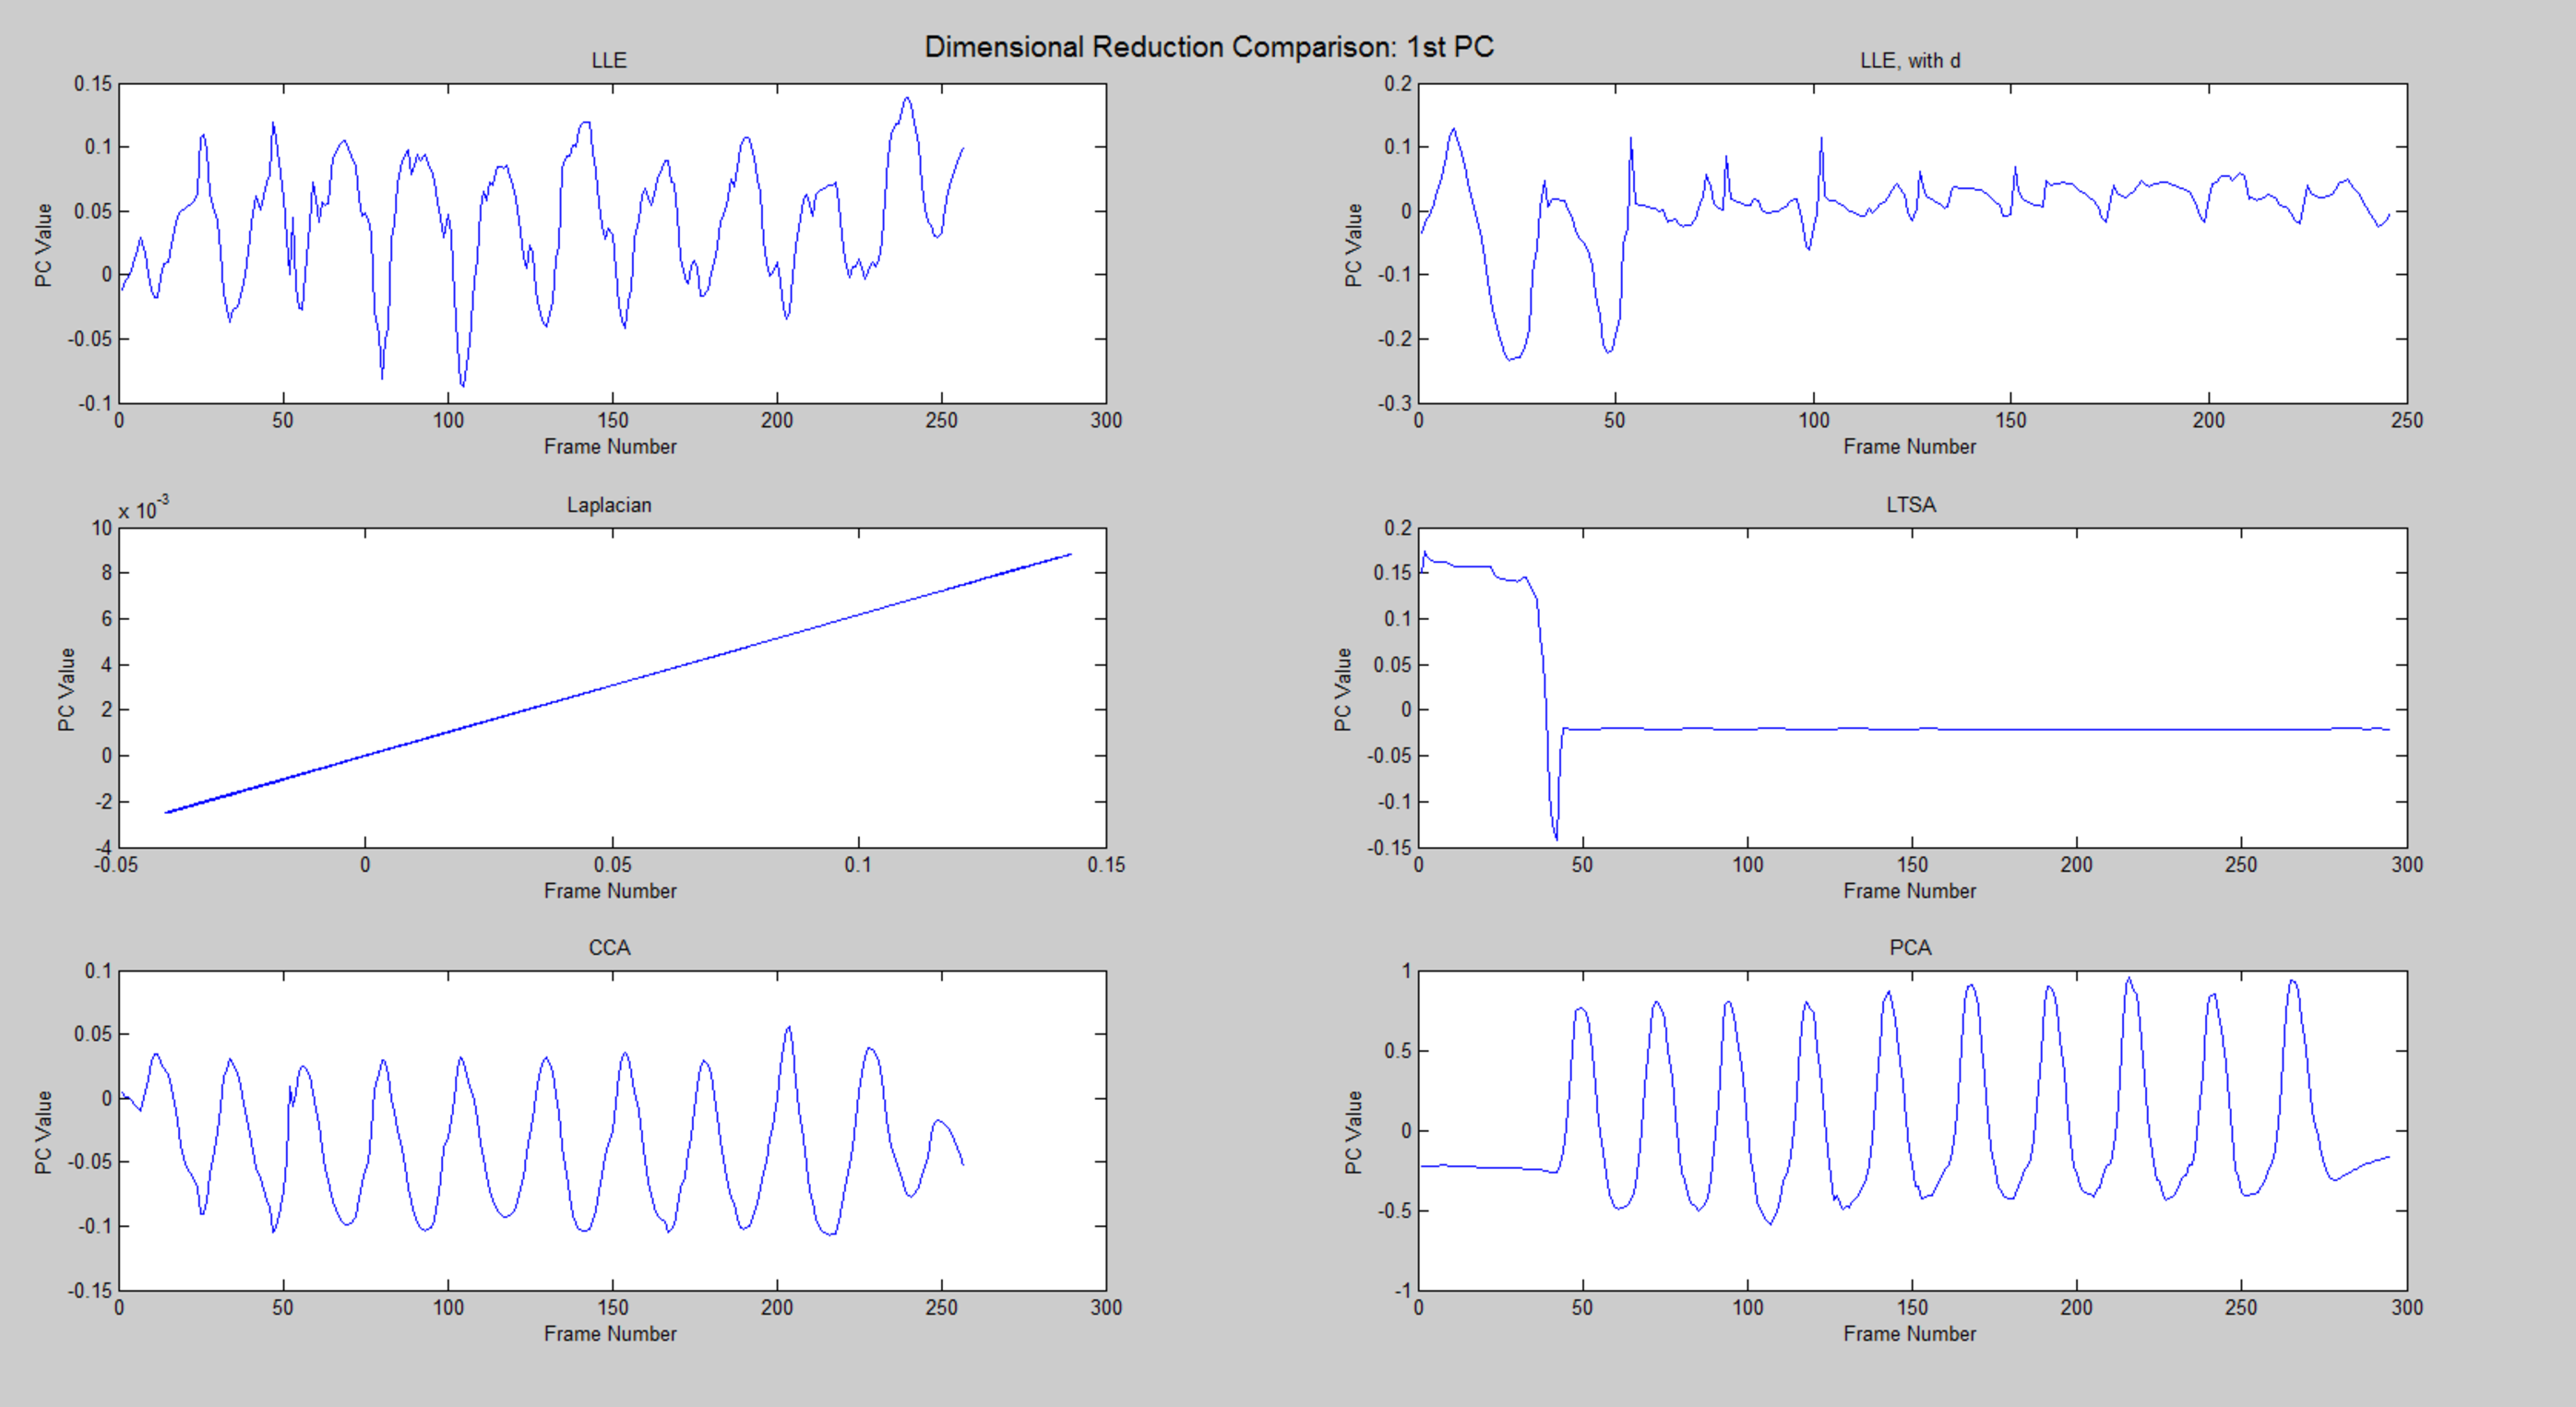
\includegraphics[height=0.25\textheight]{fig04/drcomp.pdf}
    \mycaption[Kinect Device]{1st PC comparison}
    \label{fig:drcomp}
\end{figure}
\begin{figure}[h]
    \centering
    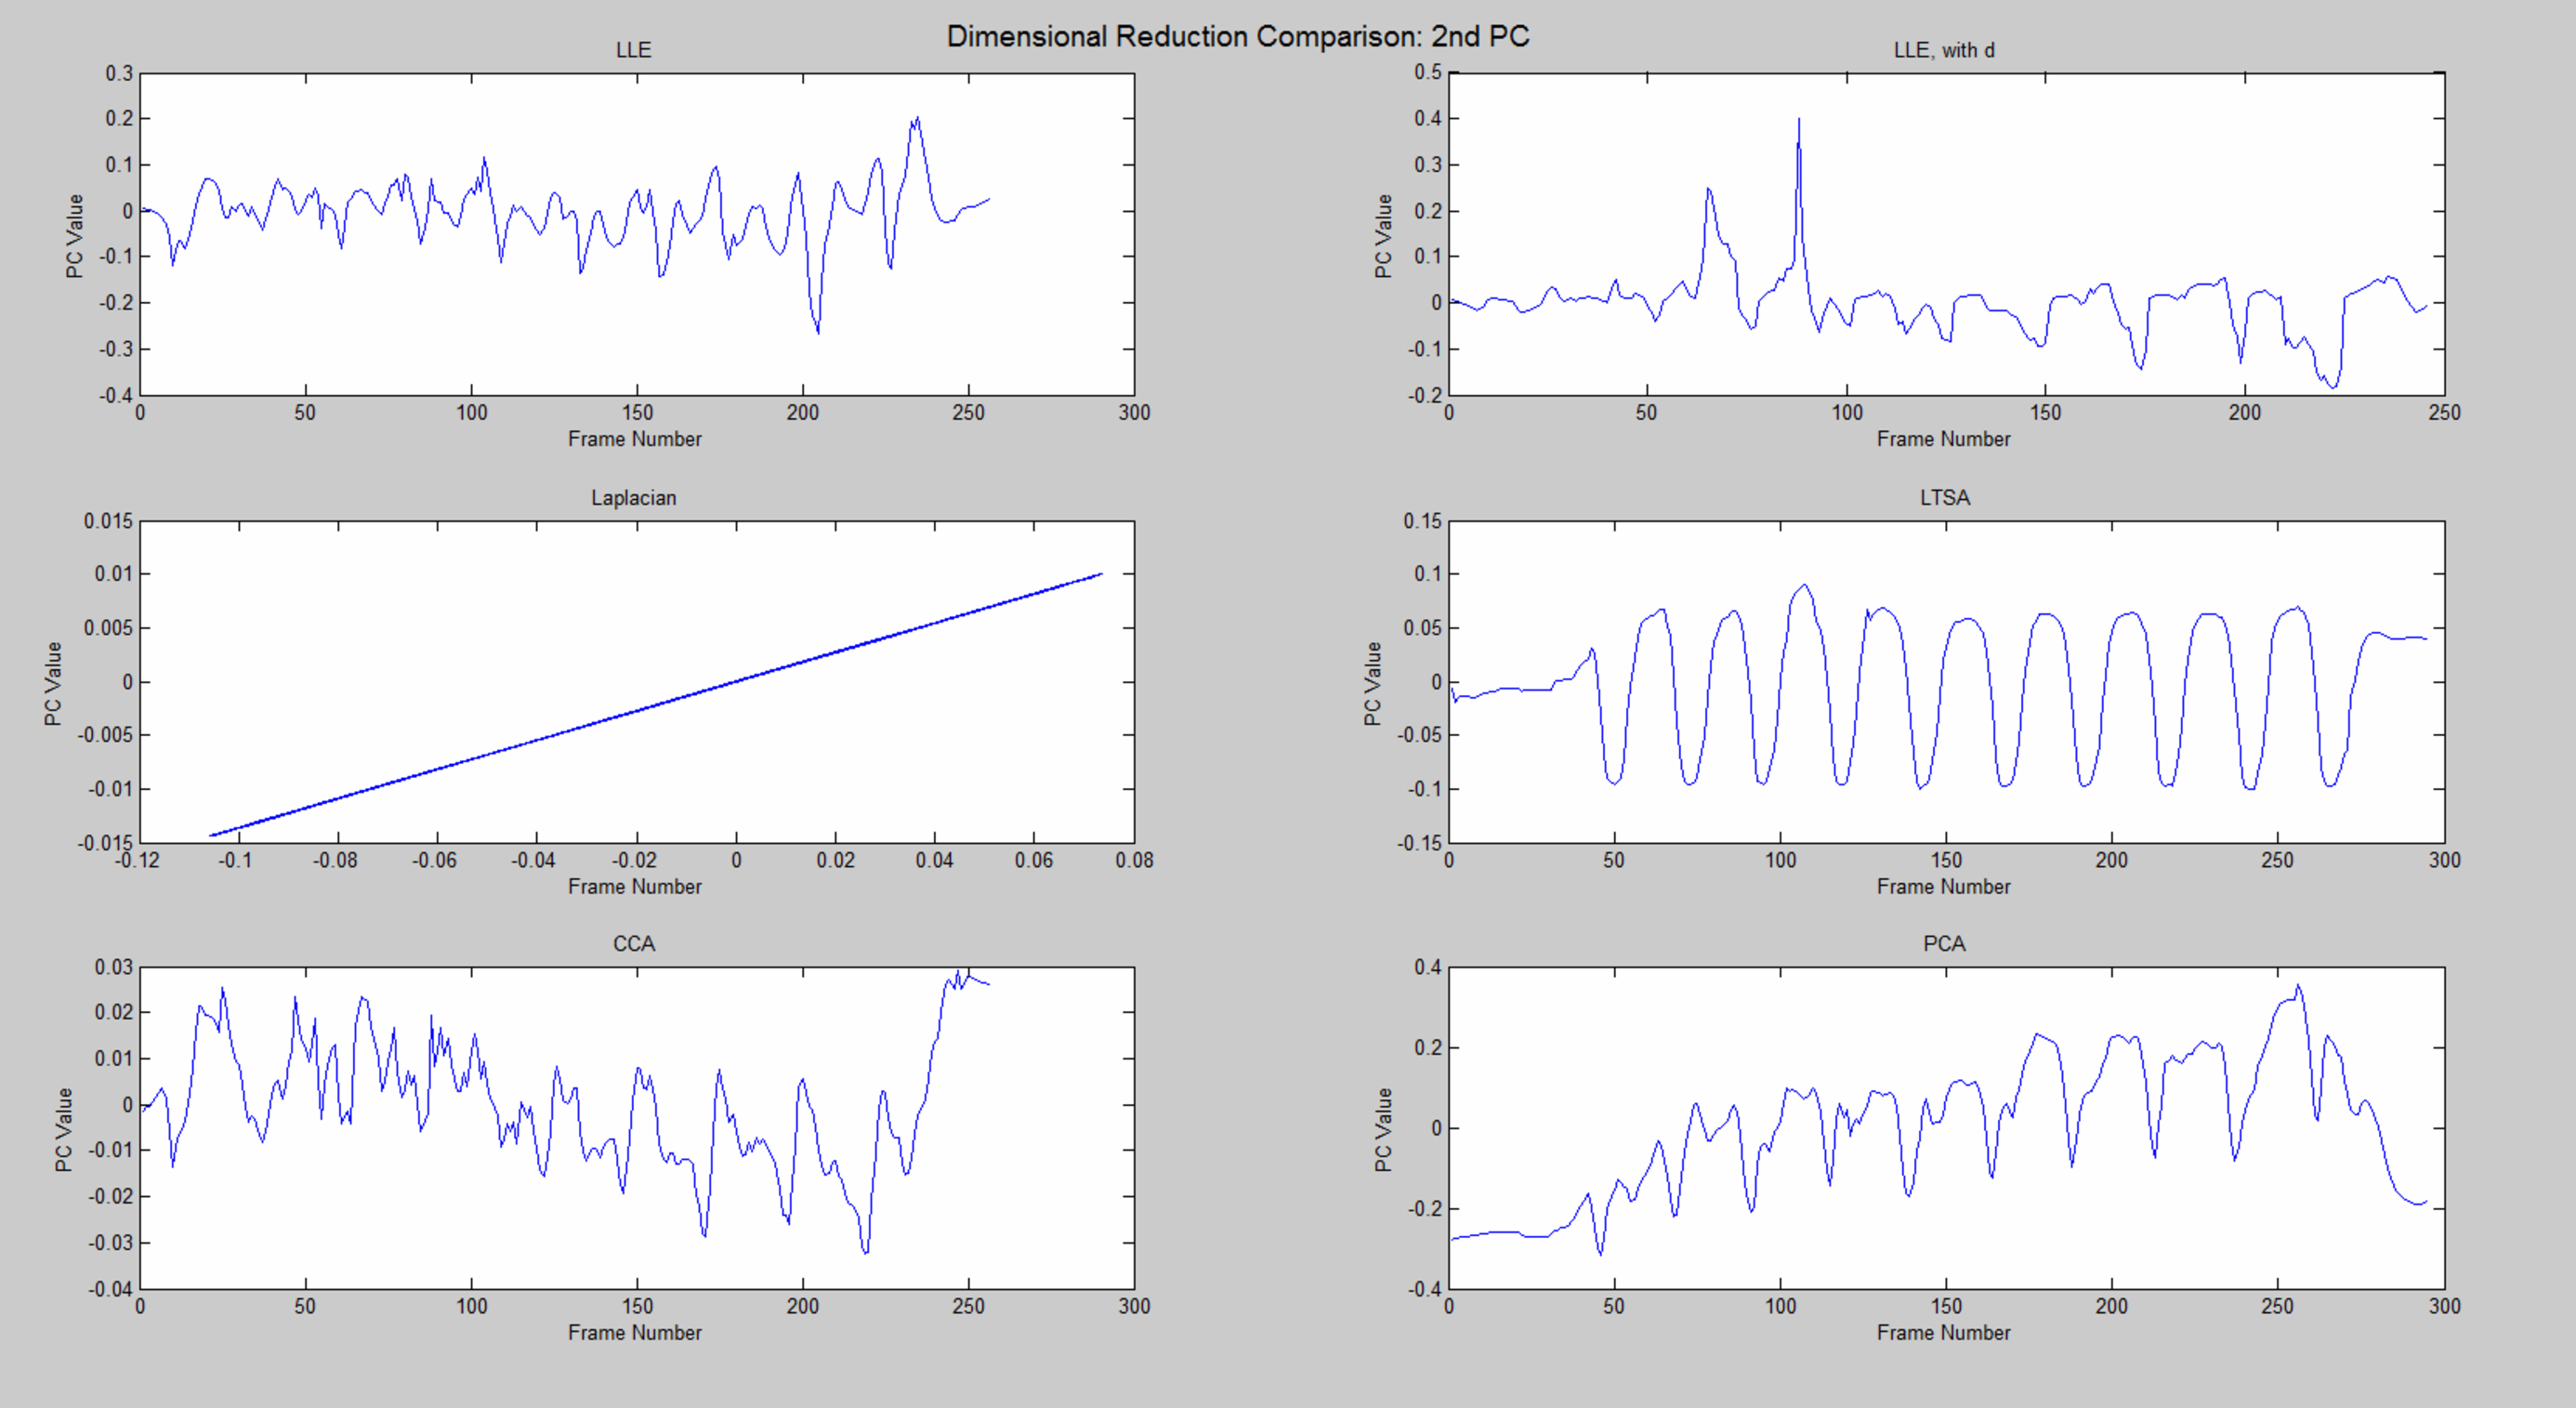
\includegraphics[height=0.25\textheight]{fig04/drcomp2.pdf}
    \mycaption[Kinect Device]{2nd PC comparison}
    \label{fig:drcomp}
\end{figure}

We can see from the first principal component plotted from multiple dimensionality reduction method that PCA does in fact give the most useful results, followed closely by CCA. If we then look at the second {\bf principal components} we can see that PCA performs second to LTSA but since LTSA performs poorly for the first component it makes PCA the obvious choice.

Despite PCA being an older, simple technique than more modern techniques such as diffusion maps it actually produced the most uniform, cyclical signal for the first component making it an obvious choice.

\begin{figure}[h]
\centering
\begin{minipage}{6.0cm}
    \centering
    \subtop[]{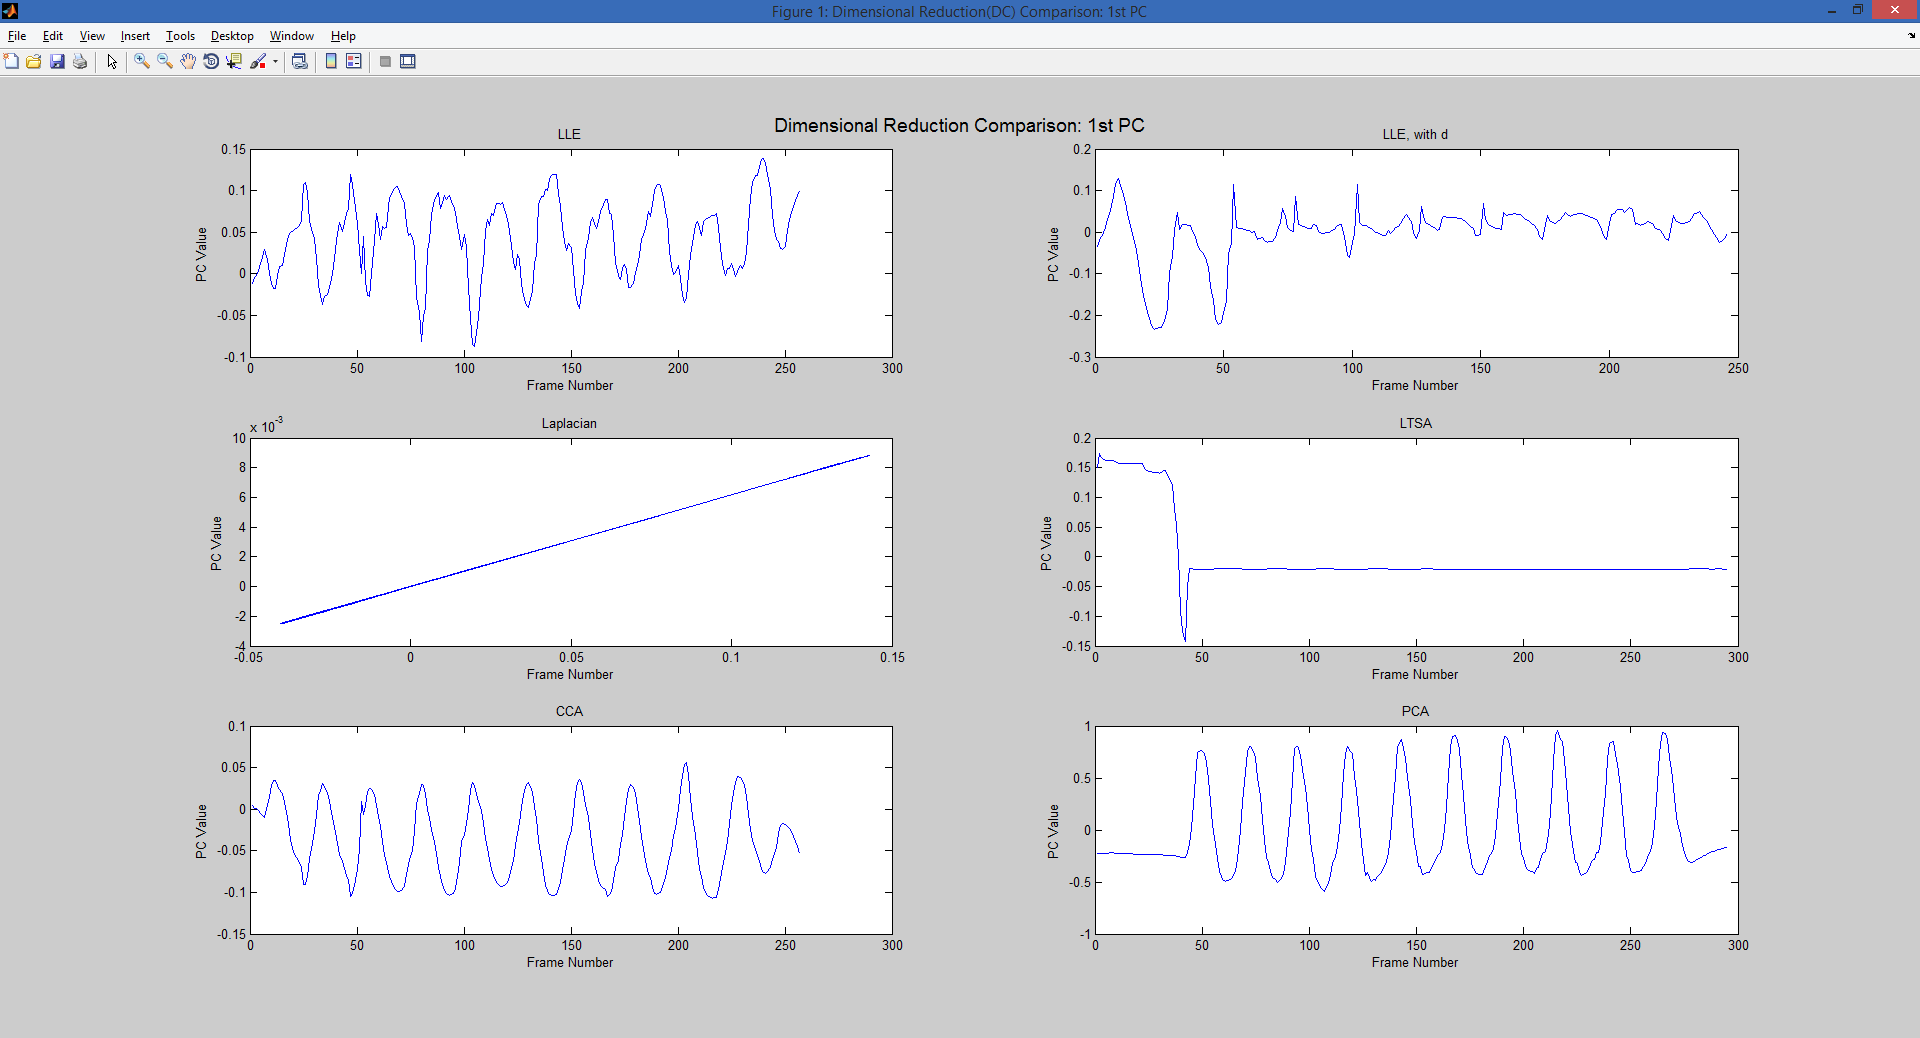
\includegraphics[height=0.25\textheight]{fig04/fig08}}
    \label{fig:kinect}
\end{minipage}
\hspace{0.5cm}
\begin{minipage}{6.0cm}
    \centering
    \subtop[]{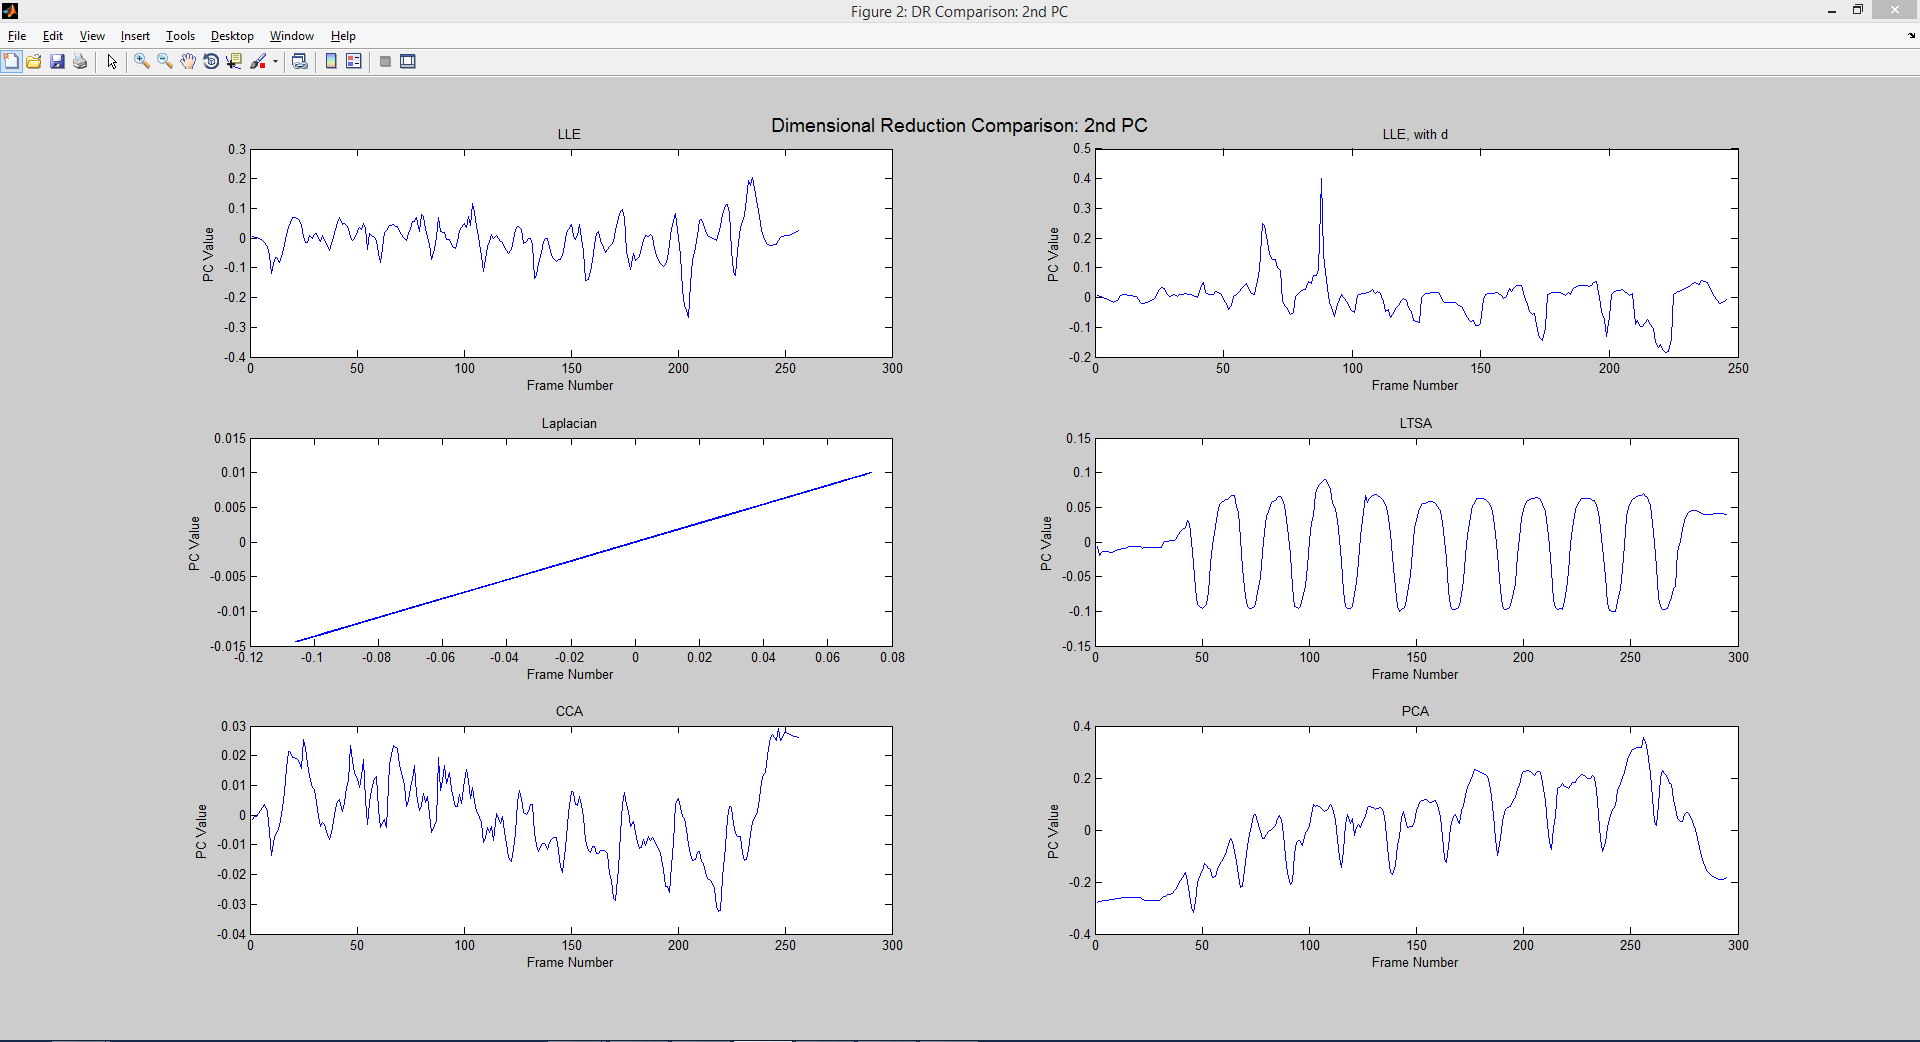
\includegraphics[height=0.25\textheight]{fig04/fig09}}
    \label{fig:kinect2}
\end{minipage}
\begin{minipage}{6.0cm}
    \centering
    \subtop[]{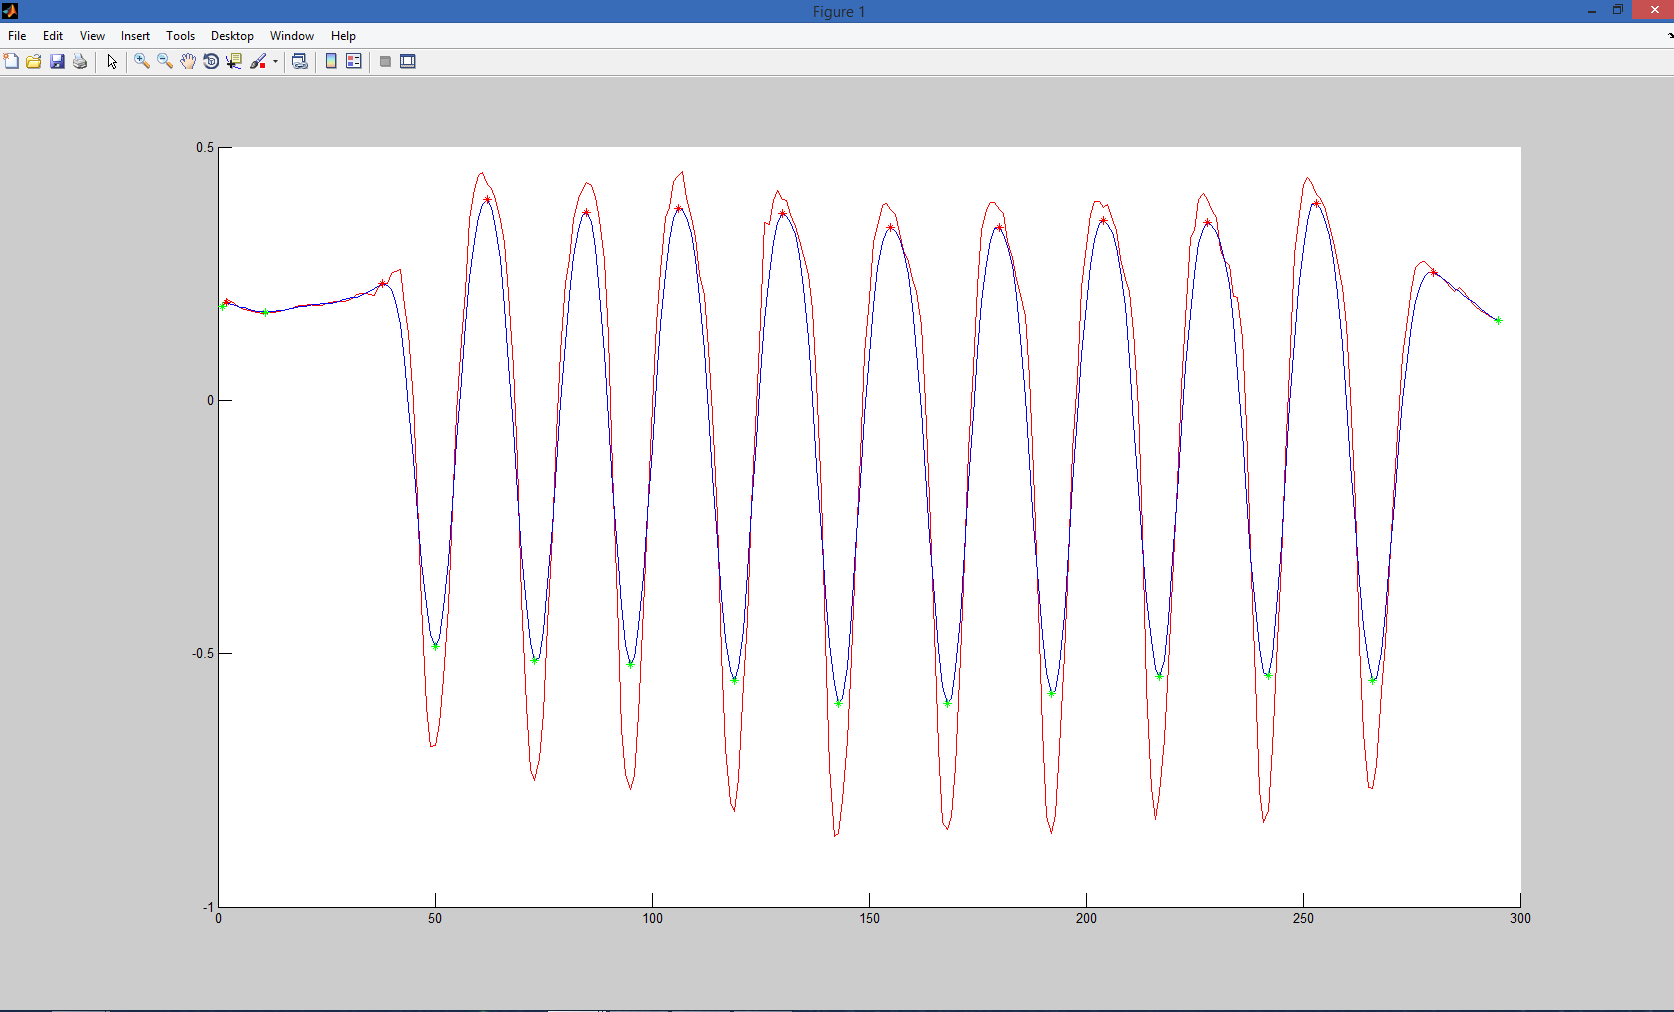
\includegraphics[height=0.25\textheight]{fig04/fig10}}
    \label{fig:kinect2}
\end{minipage}
\mycaption[WAT]{(a) Comparison of Dimensionality Reduction Techniques. PLotting first and second principal components.}
\end{figure}

Now lets see the first Principal Component (from PCA) for each punch.
TALK about normalisation of data.
Talk about getting better data.


\subsection{Punch Segmentation Algorithm}
After failing to find a way to automatically segment punches using existing methods It became apparent that a custom algorithm will be needed for this task, which can be broken down into several steps.

\begin{enumerate}[noitemsep]
  \item Perform PCA on raw data.
  \item Smooth the principal coefficients.
  \item Find the local maxima and minima for the punch sequence.
  \item Remove erroneous Minima\/Maxima using heuristic rules.
  \item Take a number of evenly spaced samples from between two maximum points, the length of one punch.
  \item Fetch all PCA components that correspond to the time the samples were taken.
  \item Train classifier on new data.
\end{enumerate}

Each frame representing 20 joint positions is reduced from 60 dimensions to 3 principal components per frame. Next the principal components are smoothed to remove any {\bf wrong minima/maxima} which would prevent the automated segmentation of punches. All remaining maxima are then passed through a set of heuristic rules that checks the location of a maxima point relative to it's neighbourhood points to determine if it is legitimate. The simplest form of this is using the Pythagorean theorem to calculate the distance between a maxima and it's neighbours, if the distance is too small it is clear that one of the points is erroneous and that only one of these will be necessary for segmentation. Likewise if a neighbour is too far away it becomes obvious that one of the maxima is incorrect and needs to be removed.\textcolor{red}{image showing points really far down compared to baseline} Thresholding is also used for each punch, with all maxima below a certain threshold removed since the cyclical signature of the punch guarantees the end of the punch will be approximately close to the end of the last punch.

 I decided the best way to do this was to smooth the signal and use local maxima/minima as a means of successfully segmenting the beginning and end of each punch. 


\begin{figure}[h]
\centering
\begin{minipage}{6.0cm}
    \centering
    \subtop[]{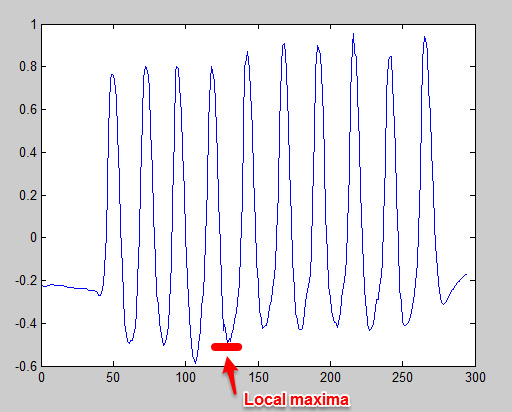
\includegraphics[height=0.25\textheight]{fig04/fig02}}
    \label{fig:kinect}
\end{minipage}

\hspace{0.5cm}
\begin{minipage}{6.0cm}
    \centering
    \subtop[]{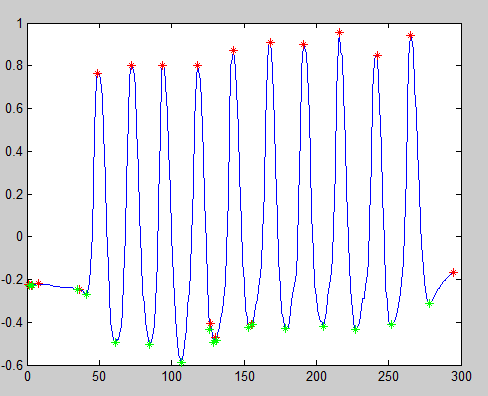
\includegraphics[height=0.25\textheight]{fig04/fig04}}
    \label{fig:kinect2}
\end{minipage}
\begin{minipage}{3.5cm}
    \centering
    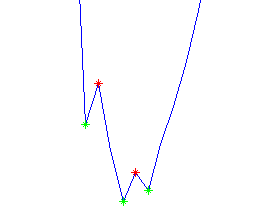
\includegraphics[height=0.15\textheight]{fig04/fig05}
    \label{fig:kinect3}
\end{minipage}
\mycaption[WAT]{(a) Periodic punch signal over time (frame number).(b) Periodic signal with local maxima/minima labelled. (c) Close up of local maxima/minima.}
\end{figure}